\section{Remap}
Doordat schermen in 3d gedraaid zijn is er nood aan een correctie van het perspectief. Dit is onder meer nodig voor het lezen van de barcode en het displayen van foto's. Het basis algorithme die hiervoor gebruikt wordt zal source en destination corners gebruiken als input. Deze corners zijn de start en eind hoeken, de foto zal dus naar de destination corners worden gerokken. Er zal per corner array een matrix worden berekent. Eerst worden de coefficienten berekent.
$$ \begin{bmatrix}
x_1 & x_2 & x_3 \\ y_1 & y_2 & y_3 \\ 1 & 1 & 1
\end{bmatrix} \begin{bmatrix}
\lambda \\ \mu \\ \tau
\end{bmatrix} =
\begin{bmatrix}
x_4 \\ y_4 \\ 1
\end{bmatrix}
$$
$$ \begin{bmatrix}
\lambda \\ \mu \\ \tau
\end{bmatrix} =\begin{bmatrix}
x_1 & x_2 & x_3 \\ y_1 & y_2 & y_3 \\ 1 & 1 & 1
\end{bmatrix}^{-1}
\begin{bmatrix}
x_4 \\ y_4 \\ 1
\end{bmatrix}
$$
Daarna wordt de 3x3 matrix geschaald met de gevonden coefficienten.
$$
\begin{bmatrix}
\lambda x_1 & \mu x_2 & \tau x_3 \\ \lambda y_1 & \mu y_2 & \tau y_3 \\ \lambda & \mu & \tau
\end{bmatrix}
$$
De twee matrices A en B, respecitivelijk met de source en destination corners, worden gebruikt om de transformatie matrix te berekenen.
$$ C = AB^{-1}$$
Deze zal elke destination pixel een de source pixel geven aan de hand van:
$$
\begin{bmatrix}
x' \\ y' \\ z'
\end{bmatrix} = C\begin{bmatrix}
x \\ y \\ 1
\end{bmatrix}
$$
$$x_{nieuw} = x'/z'$$  
$$y_{nieuw} = y'/z'$$
Een simpel algorithme zal over alle pixels (dit zijn width $ * $ height pixels) gaan en de correct kleur toevoegen.Zie figuur \ref{mappedfoto}.\cite{map}
\begin{figure}
\center
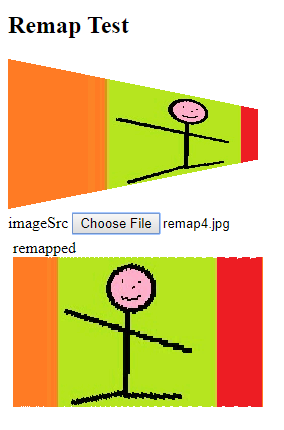
\includegraphics[scale=1]{remapEx}
\caption{Voorbeeld van een remapped foto}
\label{mappedfoto}
\end{figure}




